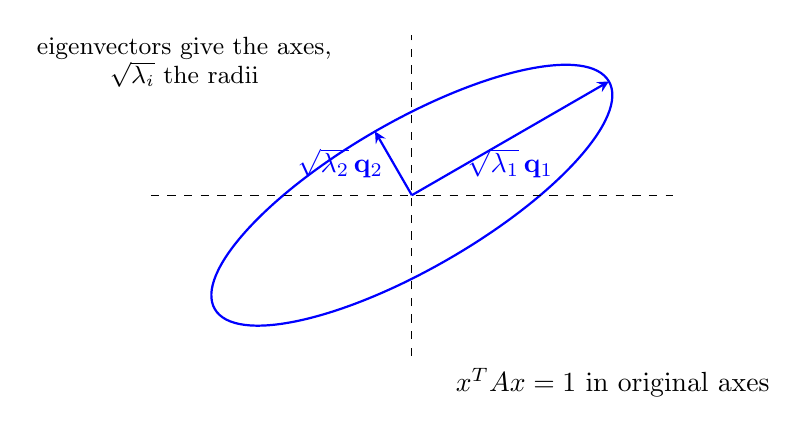
\begin{tikzpicture}[scale=0.85,>=stealth]
\begin{scope}[rotate=30]
\draw[blue,thick] (0,0) ellipse (3.4 and 1.1);
\draw[->,thick,blue] (0,0)--(3.4,0) node[midway,below]{$\sqrt{\lambda_1}\,\mathbf q_1$};
\draw[->,thick,blue] (0,0)--(0,1.1) node[midway,left]{$\sqrt{\lambda_2}\,\mathbf q_2$};
\end{scope}
\draw[dashed] (-3.9,0)--(3.9,0); \draw[dashed] (0,-2.4)--(0,2.4);
\node at (3.0,-2.8) {$x^{T}Ax=1$ in original axes};
\node at (-3.4,2.2) {\small eigenvectors give the axes,};
\node at (-3.4,1.8) {\small $\sqrt{\lambda_i}$ the radii};
\end{tikzpicture}
